\section{Auswertung}
\label{sec:Auswertung}

\subsection{Energieverteilung der Elektronen}
\label{ssec:auswwertung_elektronen}

Um die Energieverteilung der Elektronen bei konstanter Beschleunigungsspannung $U_B=\SI{11}{\volt}$ darzustellen, wurde mit einem XY-Schreiber ein Graph gezeichnet. 
Dieser ist in \autoref{fig:originaldaten_elektronen} zu sehen.

Die Messung wurde bei einer Temperatur von ungefähr $\SI{25}{\celsius}$ durchgeführt.
Bei dieser Temperatur ergibt sich über \autoref{eq:wegl} und \autoref{eq:dampfdr} die mittlere freie Weglänge zu
\begin{equation*}
    \bar{w} = \SI{0.55}{\centi\metre} \, .
\end{equation*}
Die Beschleunigungsstrecke der hier verwendeten Apperatur beträgt etwa $a=\SI{1}{\centi\metre}$.
Also ist $\bar{w}$ nicht wesentlich kleiner als $a$ und es kommt nur zu wenigen Zusammenstößen.

Aus dem Graphen werden in konstantem Abstand auf der X-Achse Punkte abgelesen, indem auf dem Millimeterpapier die Anzahl der Kästchen in X- und Y-Richtung zum nächsten Punkt gezählt werden. ($\Delta x$ und $\Delta y$ in \autoref{tab:elektronen})
Aus diesen Abständen in Kästchen werden die Abstände in Volt bzw. Nanoampere über
\begin{align}
    \Delta U_A &= \Delta x \cdot \frac{\SI{9.4}{\volt}}{\SI{236}{Kästchen}} \\
    \Delta I_A &= \Delta y \cdot \frac{\SI{60}{\nano\ampere}}{\SI{145}{Kästchen}}
\end{align}
berechnet.
Dann werden die tatsächlichen Werte über
\begin{align}
    U_{A,k} &= U_{A,k-1} + \Delta U_{A,k-1} &\text{mit\hspace{1cm}} U_{A,0} &= \SI{0.6}{\volt} \\
    I_{A,k} &= I_{A,k-1} - \Delta I_{A,k-1} &\text{mit \hspace{1cm}} I_{A,0} &= \SI{105}{\nano\ampere}
\end{align}
berechnet.
Alle gemessenen und berechneten Werte sind in \autoref{tab:elektronen} aufgelistet.
Außerdem wird je ein Plot der integralen Energieverteilung (\autoref{fig:plot_elektronen}) und der differentiellen Energieverteilung (\autoref{fig:plot_elektronen_diff}) erstellt.

Das Kontaktpotential kann hier nicht bestimmt werden, da die integrale Energieverteilung nicht abgeflacht ist.

\begin{table}
    \centering
    \caption{Abgelesene und berechnete Werte der Energieverteilung aus \autoref{fig:originaldaten_elektronen}}
    \sisetup{
        table-format=1.2
    }
    \resizebox{0.7\textwidth}{!}{%
        \begin{tabular}{S[table-format=2.0] S S S[table-format=2.0] S S[table-format=3.2]}
            \toprule
            \tableSI{\Delta x}{Kästchen} & \tableSI{\Delta U_A}{\volt} & \tableSI{U_A}{\volt} & \tableSI{\Delta y}{Kästchen} & \tableSI{\Delta I_A}{\nano\ampere} & \tableSI{I_A}{\nano\ampere} \\
            \midrule
            6 & 0.24 & 0.60 & 4 & 1.66 & 105.00 \\
            10 & 0.40 & 0.84 & 4 & 1.66 & 103.34 \\
            10 & 0.40 & 1.24 & 4 & 1.66 & 101.69 \\
            10 & 0.40 & 1.64 & 4 & 1.66 & 100.03 \\
            10 & 0.40 & 2.03 & 4 & 1.66 & 98.38 \\
            10 & 0.40 & 2.43 & 4 & 1.66 & 96.72 \\
            10 & 0.40 & 2.83 & 4 & 1.66 & 95.07 \\
            10 & 0.40 & 3.23 & 4 & 1.66 & 93.41 \\
            10 & 0.40 & 3.63 & 4 & 1.66 & 91.76 \\
            10 & 0.40 & 4.03 & 5 & 2.07 & 90.10 \\
            10 & 0.40 & 4.42 & 5 & 2.07 & 88.03 \\
            10 & 0.40 & 4.82 & 5 & 2.07 & 85.97 \\
            10 & 0.40 & 5.22 & 5 & 2.07 & 83.90 \\
            10 & 0.40 & 5.62 & 6 & 2.48 & 81.83 \\
            10 & 0.40 & 6.02 & 6 & 2.48 & 79.34 \\
            10 & 0.40 & 6.42 & 6 & 2.48 & 76.86 \\
            10 & 0.40 & 6.81 & 6 & 2.48 & 74.38 \\
            10 & 0.40 & 7.21 & 7 & 2.90 & 71.90 \\
            10 & 0.40 & 7.61 & 7 & 2.90 & 69.00 \\
            10 & 0.40 & 8.01 & 8 & 3.31 & 66.10 \\
            10 & 0.40 & 8.41 & 9 & 3.72 & 62.79 \\
            10 & 0.40 & 8.81 & 10 & 4.14 & 59.07 \\
            10 & 0.40 & 9.20 & 11 & 4.55 & 54.93 \\
            10 & 0.40 & 9.60 & 13 & 5.38 & 50.38 \\
            &  & 10.00 &  &  & 45.00 \\
            \bottomrule
        \end{tabular}
    }
    \label{tab:elektronen}
\end{table}

\begin{figure}
    \centering
    \includegraphics[width=\textwidth]{build/plot_elektronen.pdf}
    \caption{Plot der integralen Energieverteilung der Elektronen}
    \label{fig:plot_elektronen}
\end{figure}

\begin{figure}
    \centering
    \includegraphics[width=\textwidth]{build/plot_elektronen_diff.pdf}
    \caption{Plot der differentiellen Energieverteilung der Elektronen}
    \label{fig:plot_elektronen_diff}
\end{figure}


\subsection{Franck-Herz-Kurve und Anregungsenergie von Hg}
\label{ssec:auswertung_franck-hertz}

Bei konstanter Bremsspannung $U_A = \SI{1}{\volt}$  wurde mit einem XY-Schreiber der Auffängerstrom gegen die Beschleunigungsspannung aufgetragen. (siehe \autoref{fig:originaldaten_franck-hertz}) 

Die Messung wurde bei einer Temperatur von ungefähr $\SI{180}{\celsius}$ durchgeführt.
Bei dieser Temperatur ergibt sich über \autoref{eq:wegl} und \autoref{eq:dampfdr} die mittlere freie Weglänge zu
\begin{equation*}
    \bar{w} = \SI{2.05e-4}{\centi\metre} \, .
\end{equation*}
Die Beschleunigungsstrecke der hier verwendeten Apperatur beträgt etwa $a=\SI{1}{\centi\metre}$.
Also ist $\bar{w}$ wesentlich kleiner als $a$ und es kommt zu genug Zusammenstößen, sodass eine Franck-Hertz-Kurve entstehen kann.

Hier werden die Abstände $\Delta x$ der relativen Maxima abgelesen und mit
\begin{equation}
    \Delta U_B = \Delta x \cdot \frac{\SI{60}{\volt}}{\SI{194}{Kästchen}}
\end{equation}
in Spannungsabstände umgerechnet.
Die abgelesenen und berechneten Werte sind in \autoref{tab:franck-hertz} aufgelistet.

\begin{table}
    \centering
    \caption{Abgelesene und daraus berechnete Abstände der relativen Maxima der Franck-Hertz-Kurve \autoref{fig:franck-hertz}}
    \begin{tabular}{S[table-format=2.0] S[table-format=1.2]}
        \toprule
        \tableSI{\Delta x}{Kästchen} & \tableSI{\Delta U_B}{\volt} \\
        \midrule
        16 & 4.95 \\
        17 & 5.26 \\
        18 & 5.57 \\
        18 & 5.57 \\
        \bottomrule
    \end{tabular}
    \label{tab:franck-hertz}
\end{table}

\begin{figure}
    \centering
    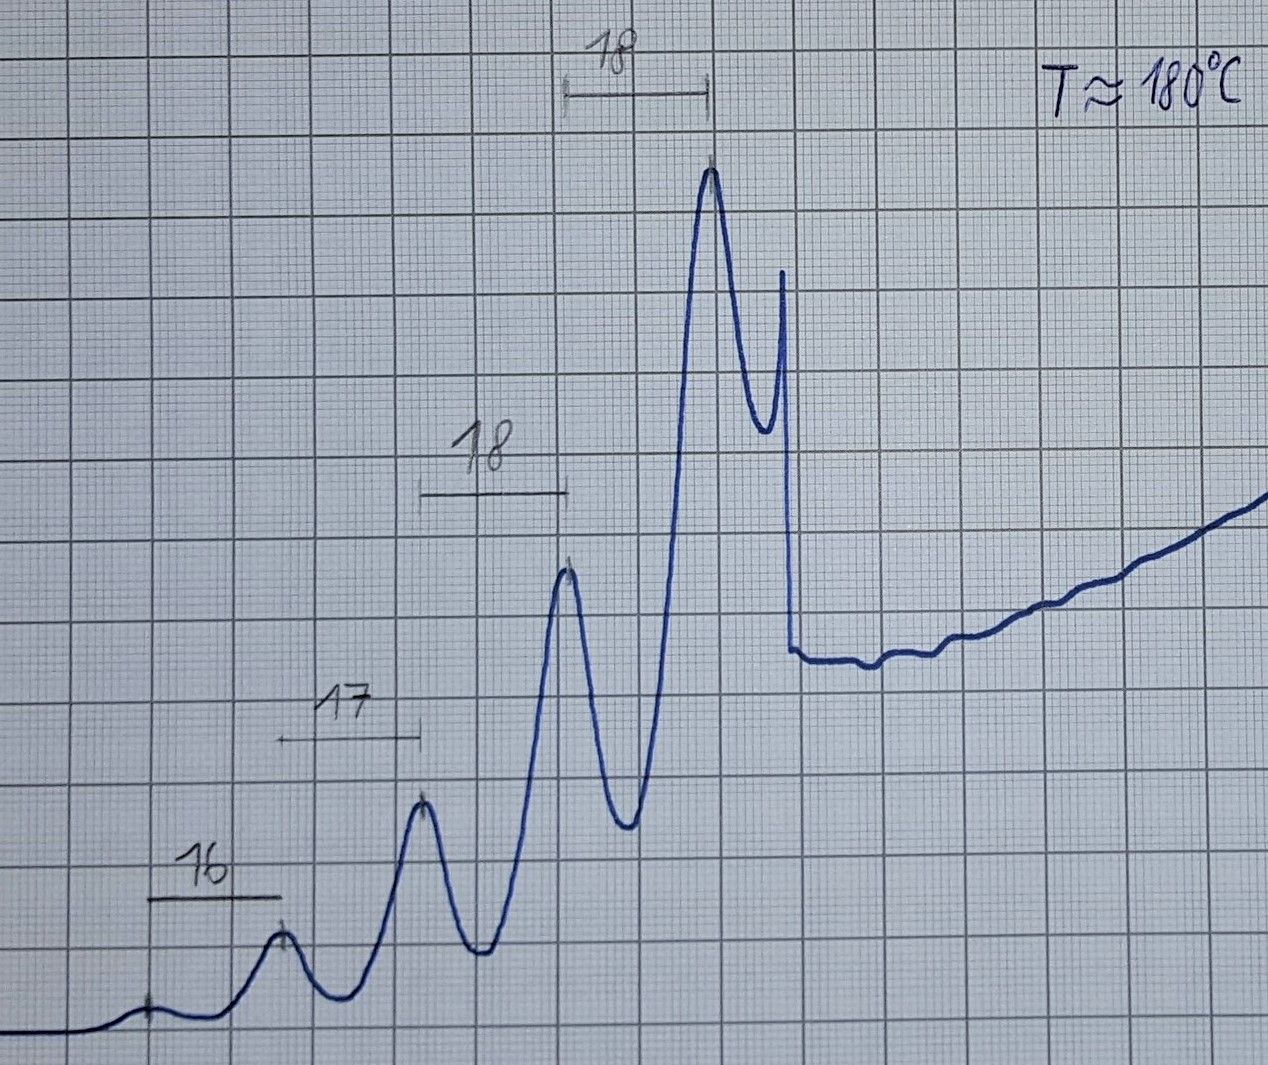
\includegraphics[width=\textwidth]{images/franck-hertz.jpg}
    \caption{mit X-Y-Schreiber aufgenommene Franck-Hertz-Kurve}
    \label{fig:franck-hertz}
\end{figure}

Anzumerken sei, dass die Elektronen durch elastische Stöße Energie verlieren und dadurch die Franck-Hertz Kurve abgeflacht wird.
Da jedoch hier nur die Abstände der Maxima in Bezug auf die Beschleunigungsspannung für Berechnungen verwendet werden, muss dieser Effekt hier nicht beachtet werden.

Aus diesen Werten wird nun der mittlere Abstand der Maxima und der entsprechende Fehler des Mittelwerts berechnet.
\begin{equation*}
    \bar{\Delta U_B} = \SI{5.34+-0.15}{\volt}
\end{equation*}
Nach \autoref{eq:ueins} und $e_0 \cdot \SI{1}{\volt}=\SI{1}{\electronvolt}$ ist die erste Anregungsenergie des Hg-Atoms gerade
\begin{equation*}
    E_{01} = \SI{5.34+-0.15}{\electronvolt} \, .
\end{equation*}
Daraus lässt sich nach \autoref{eq:quant} die Wellenlänge $\lambda$ der emitierten elektromagnetischen Strahlung über
\begin{equation}
    \lambda = \frac{h \cdot c}{E_{01}}
\end{equation}
zu
\begin{equation*}
    \lambda = \SI{2.32+-0.06e-07}{\metre}
\end{equation*}
berechnen. 